\documentclass[12pt]{beamer}
\usepackage[utf8]{inputenc}
\usepackage{graphicx}
\usepackage{float}
\graphicspath{ {images/} }

\usepackage{mathtools}
\usepackage{amsfonts, amsmath, amsthm, amssymb}
\usepackage{adjustbox}
\usepackage{tabularx}


%\newtheorem{thm}{Theorem}[section]
%\newtheorem{lemma}[thm]{Lemma}
%
%\theoremstyle{definition}
%\newtheorem{defin}[thm]{Definition}
%
%\theoremstyle{remark}
%\newtheorem{rem}[thm]{Remark}
%\newtheorem{ex}[thm]{Example}

\usepackage{inputenc}
\usepackage{tikz}
\usetikzlibrary{tikzmark}
\usetikzlibrary{shapes.geometric, arrows}

\setbeamertemplate{frametitle}
  {\begin{centering}\smallskip
   \insertframetitle\par
   \smallskip\end{centering}}
\setbeamertemplate{itemize item}{$\bullet$}
\setbeamertemplate{navigation symbols}{}
\setbeamertemplate{footline}[text line]{%
    \hfill\strut{%
        \scriptsize\sf\color{black!60}%
        \quad\insertframenumber
    }%
    \hfill
}

% Define some colors:
\definecolor{DarkFern}{HTML}{407428}
\definecolor{DarkCharcoal}{HTML}{4D4944}
\colorlet{Fern}{DarkFern!85!white}
\colorlet{Charcoal}{DarkCharcoal!85!white}
\colorlet{LightCharcoal}{Charcoal!50!white}
\colorlet{AlertColor}{orange!80!black}
\colorlet{DarkRed}{red!70!black}
\colorlet{DarkBlue}{blue!70!black}
\colorlet{DarkGreen}{green!70!black}
% Use the colors:
\setbeamercolor{title}{fg=Fern}
\setbeamercolor{frametitle}{fg=Fern}
\setbeamercolor{normal text}{fg=Charcoal}
\setbeamercolor{block title}{fg=black,bg=Fern!25!white}
\setbeamercolor{block body}{fg=black,bg=Fern!25!white}
\setbeamercolor{alerted text}{fg=AlertColor}
\setbeamercolor{itemize item}{fg=Charcoal}

\AtBeginSubsection[]
{
  \begin{frame}
    \frametitle{ }
    \tableofcontents[currentsection, currentsubsection]
  \end{frame}
}

\AtBeginSection[]
{
  \begin{frame}
    \frametitle{ }
    \tableofcontents[currentsection, currentsubsection]
  \end{frame}
}


\tikzstyle{startstop} = [rectangle, rounded corners, minimum width=3cm, minimum height=1cm,text centered, draw=black, fill=red!30]
\tikzstyle{io} = [trapezium, minimum width=1.5cm, minimum height=1cm, text centered, draw=black, fill=blue!30]
\tikzstyle{process} = [rectangle, minimum width=3cm, minimum height=1cm, text centered, draw=black, fill=orange!30]
\tikzstyle{decision} = [diamond, minimum width=3cm, minimum height=1cm, text centered, draw=black, fill=green!30]
\tikzstyle{arrow} = [thick,->,>=stealth]

\title{OTP and AES: A Historical Transition Between two Systems of Cryptography}
\author{Valdemar Thanner \\ Supervised by Mr. Bernhard Keller\\
Linguistic supervision by Ms. Margrit Oetiker}
\date{06.03.2017}
\institute{Kantonsschule Zug}


\begin{document}

\frame{\titlepage}

\begin{frame}{Overview}
\tableofcontents
\end{frame}

\section{A Brief Overview of Cryptography}

\begin{frame}
\frametitle{What is Cryptography?}
\begin{center}
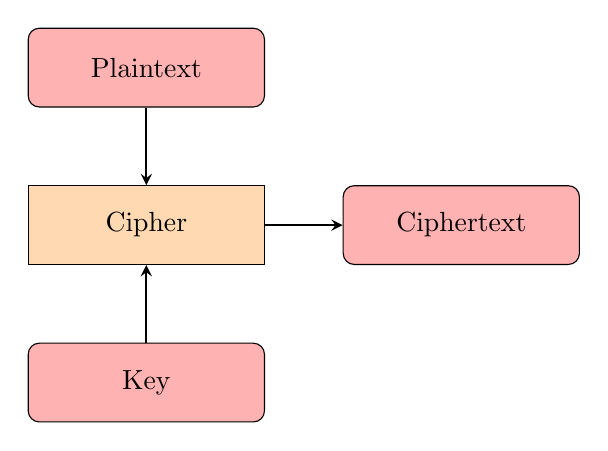
\begin{tikzpicture}[node distance=2cm]
\node (plaintext) [startstop] {Plaintext};
\node (cipher) [process, below of = plaintext] {Cipher};
\node (key) [startstop, below of = cipher] {Key};
\node (ciphertext) [startstop, right of = cipher, xshift = 2cm] {Ciphertext};
\draw [arrow] (plaintext) -- (cipher);
\draw [arrow] (key) -- (cipher);
\draw [arrow] (cipher) -- (ciphertext);
\end{tikzpicture}
\end{center}
\uncover<2->{
\begin{itemize}
\item "The art of writing or solving codes"
\item The study of creating or breaking ciphers
\end{itemize}
}
\end{frame}

\section{OTP}

\begin{frame}
\frametitle{OTP: The One Time Pad}
\begin{itemize}
\item Great historical impact
\item Basis for or important part of many of today's modern algorithms
\item The key must be disposed of securely after being used once
\item Symmetrical cipher: Keeping of a shared secret
\end{itemize}
\end{frame}

\begin{frame}
\frametitle{OTP: The Cipher}
\begin{columns}
\begin{column}{0.5\textwidth}
\begin{itemize}
\item Stream Cipher
\item Key length $\geq$ Message length
\item Based on modular addition
\item Perfect (forward) secrecy
\end{itemize}
\end{column}
\begin{column}{0.5\textwidth}
\includegraphics<1->[scale=0.2]{keystream.PNG}
\uncover<2->{
$b + d = 1+3 = 4 = e$
$j + t = 9+19 = 28$
\break
$(9+19) \mod 26 = 2 = c$
}
\end{column}
\end{columns}
\end{frame}

\begin{frame}
\frametitle{OTP: The Cipher}

\begin{center}
\begin{tabular}{cccccccccccc}
c & r & y & p & t & o & g & r & a & p & h & y \\
$\downarrow$ & $\downarrow$ & $\downarrow$ & $\downarrow$ & $\downarrow$ & $\downarrow$ & $\downarrow$ & $\downarrow$ & $\downarrow$ & $\downarrow$ & $\downarrow$ & $\downarrow$  \\
2 & 17 & 24 & 15 & 19 & 14 & 6 & 17 & 0 & 15 & 7 & 24 \\
\end{tabular}
\end{center}

\begin{center}
\begin{tabular}{cccccccccccc}
s & y & t & r & u & i & f & q & n & i & h & m \\
$\downarrow$ & $\downarrow$ & $\downarrow$ & $\downarrow$ & $\downarrow$ & $\downarrow$ & $\downarrow$ & $\downarrow$ & $\downarrow$ & $\downarrow$ & $\downarrow$ & $\downarrow$  \\
18 & 24 & 19 & 17 & 20 & 8 & 5 & 16 & 13 & 8 & 7 & 12 \\
\end{tabular}
\end{center}

\begin{center}
\begin{tabular}{cccccccccccc}
2+18 & 17+24 & 24+19 & 15+17 & 19+20 & 14+8 & 6+5 & 17+16 & 0+13 & 15+8 & 7+7 & 24+12 \\
$\downarrow$ & $\downarrow$ & $\downarrow$ & $\downarrow$ & $\downarrow$ & $\downarrow$ & $\downarrow$ & $\downarrow$ & $\downarrow$ & $\downarrow$ & $\downarrow$ & $\downarrow$  \\
20 & 15 & 17 & 6 & 13 & 22 & 11 & 7 & 13 & 23 & 14 & 10 \\
$\downarrow$ & $\downarrow$ & $\downarrow$ & $\downarrow$ & $\downarrow$ & $\downarrow$ & $\downarrow$ & $\downarrow$ & $\downarrow$ & $\downarrow$ & $\downarrow$ & $\downarrow$  \\
u & p & r & g & n & w & l & h & n & x & o & k
\end{tabular}
\end{center}

\end{frame}

\begin{frame}
\frametitle{OTP: A Precursor to Modern Computer-aided Cryptography}
\begin{columns}
\begin{column}{0.5\textwidth}
\begin{itemize}
\item<1-> Gilbert Vernam: Secret signaling system of 1919
\item<2-> Looping perforated tape: known-plaintext vulnerability
\item<2-> Bits: Binary digits
\end{itemize}
\end{column}
\begin{column}{0.5\textwidth}
\includegraphics<1>[scale=0.5]{VernamCipher.jpg}
\includegraphics<2->[scale=0.25]{PerforatedTape.jpg}
\end{column}
\end{columns}

\end{frame}

\section{AES: The Advanced Encryption standard}

\subsection{High Level Structure}

\begin{frame}
\frametitle{AES: Terminology}
\begin{columns}
\begin{column}{0.4\textwidth}
\begin{itemize}
\item<1-> Bit: Boolean value first conclusively described by Claude Shannon \vspace{5mm}
\item<2-> Byte: 8 Bits; can represent any number from 0-255
\end{itemize}
\end{column}
\begin{column}{0.6\textwidth}
\uncover<1->{
$0 \vee 1$
}

\uncover<2->{
\vspace{5mm}
$(2^7 + 2^6 + 2^5 + 2^4 + 2^3 + 2^2 + 2^1 + 2^0)_b$
\vspace{5mm}
$(00000011)_b = 1 \cdot 2^1 + 1 \cdot 2^0 = 3$ 
$(16 + 1)_h$
${1-9; A; B; C; D; E; F}$
$(B4)_h = 16 \cdot 11 + 4 \cdot 1 = 180$
}

\end{column}
\end{columns}

\end{frame}

\begin{frame}
\frametitle{AES: Design Goals}
\begin{itemize}
\item Confusion: Each bit of the ciphertext should depend on multiple bits of the key
\item Diffusion: The "avalanche effect", small changes to the plaintext should strongly impact the ciphertext
\item Two different implementations: Computationally or memory efficient
\end{itemize}
\end{frame}

\begin{frame}
\frametitle{AES: The Advanced Encryption Standard}
\begin{columns}
\begin{column}{0.5\textwidth}
\begin{itemize}
\item Block Cipher
\item The current N.I.S.T standard for SECRET and TOP-SECRET designated files
\item Original name: Rijndael; was selected as the successor to DES.
\end{itemize}
\end{column}
\begin{column}{0.5\textwidth}
\begin{center}
\uncover<2->{
\[ \left( \begin{array}{cccc}
a_0 & a_4 & a_8 & a_{12} \\
a_1 & a_5 & a_9 & a_{13} \\
a_2 & a_6 & a_{10} & a_{14} \\
a_3 & a_7 & a_{11} & a_{15}\end{array} \right)\] 
}
\end{center}
\end{column}
\end{columns}
\end{frame}

\begin{frame}
\frametitle{AES: High-Level Structure}

\begin{adjustbox}{max totalsize={.9\textwidth}{.7\textheight},center}
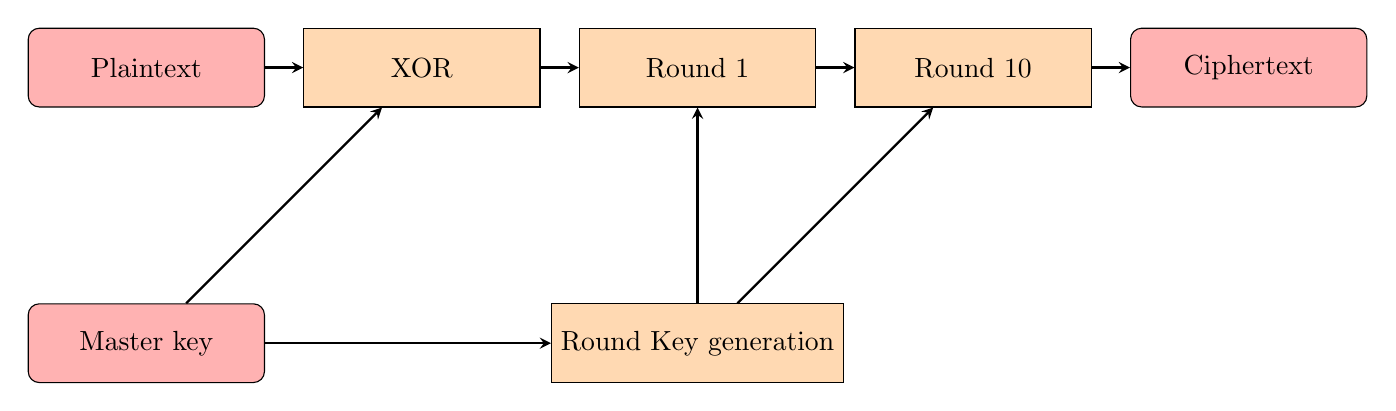
\begin{tikzpicture}[node distance=2cm ]
\node (plaintext) [startstop] {Plaintext};
\node (masterkey) [startstop, below of = plaintext, yshift=-1.5cm] {Master key};
\node (XOR) [process, right of = plaintext, xshift=1.5cm] {XOR};
\node (Roundfirst) [process, right of = XOR, xshift=1.5cm] {Round 1};
\node (Roundlast) [process, right of = Roundfirst, xshift=1.5cm] {Round 10};
\node (Ciphertext) [startstop, right of = Roundlast, xshift=1.5cm] {Ciphertext};
\node (RoundKey) [process, below of = Roundfirst, yshift=-1.5cm] {Round Key generation};
\draw [arrow] (plaintext) -- (XOR);
\draw [arrow] (XOR) -- (Roundfirst);
\draw [arrow] (Roundfirst) -- (Roundlast);
\draw [arrow] (Roundlast) -- (Ciphertext);
\draw [arrow] (masterkey) -- (RoundKey);
\draw [arrow] (masterkey) -- (XOR);
\draw [arrow] (RoundKey) -- (Roundfirst);
\draw [arrow] (RoundKey) -- (Roundlast);
\end{tikzpicture}
\end{adjustbox}
\end{frame}

\subsection{Rounds}

\begin{frame}
\frametitle{AES: Rounds}

\begin{adjustbox}{max totalsize={.9\textwidth}{.7\textheight},center}
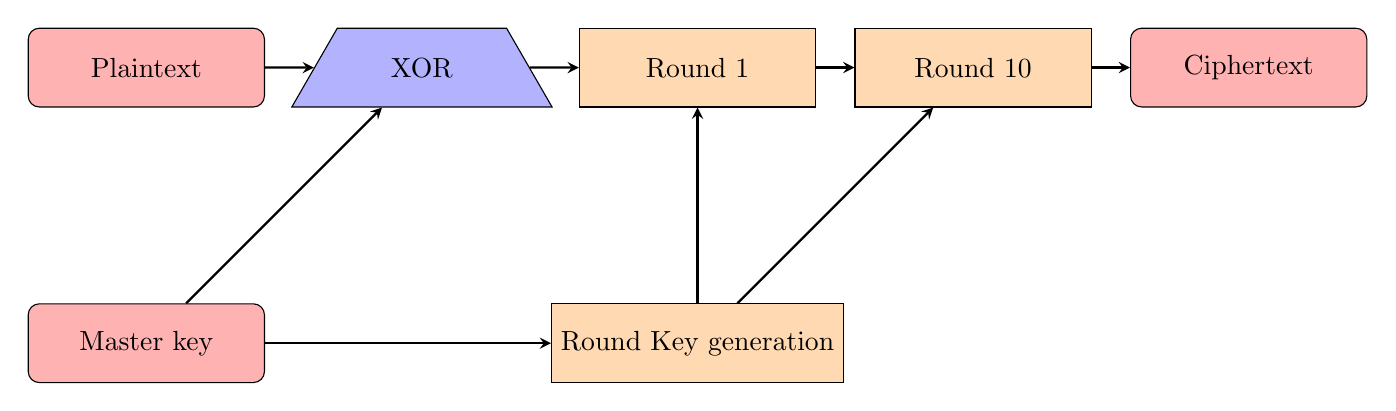
\begin{tikzpicture}[node distance=2cm]
\node (plaintext) [startstop] {Plaintext};
\node (masterkey) [startstop, below of = plaintext, yshift=-1.5cm] {Master key};
\node (XOR) [io, right of = plaintext, xshift=1.5cm] {XOR};
\node (Roundfirst) [process, right of = XOR, xshift=1.5cm] {Round 1};
\node (Roundlast) [process, right of = Roundfirst, xshift=1.5cm] {Round 10};
\node (Ciphertext) [startstop, right of = Roundlast, xshift=1.5cm] {Ciphertext};
\node (RoundKey) [process, below of = Roundfirst, yshift=-1.5cm] {Round Key generation};
\draw [arrow] (plaintext) -- (XOR);
\draw [arrow] (XOR) -- (Roundfirst);
\draw [arrow] (Roundfirst) -- (Roundlast);
\draw [arrow] (Roundlast) -- (Ciphertext);
\draw [arrow] (masterkey) -- (RoundKey);
\draw [arrow] (masterkey) -- (XOR);
\draw [arrow] (RoundKey) -- (Roundfirst);
\draw [arrow] (RoundKey) -- (Roundlast);
\end{tikzpicture}
\end{adjustbox}

\[
\pause \left( \begin{array}{cccc}
1 & 0 & 1 & 0 \\[0pt]
\bigoplus & \bigoplus & \bigoplus & \bigoplus \\[0pt]
0 & 1 & 1 & 0 \\[0pt]
= & = & = & = \\[0pt]
1 & 1 & 0 & 0 \\[0pt]
\end{array} \right)
\]

\begin{itemize}
\pause
\item bitwise logical operation; can be performed directly by the CPU
\item addition mod 2
\item can randomize biased input
\end{itemize}
\end{frame}

\begin{frame}
\frametitle{AES: Rounds}
\begin{adjustbox}{max totalsize={.9\textwidth}{.7\textheight},center}
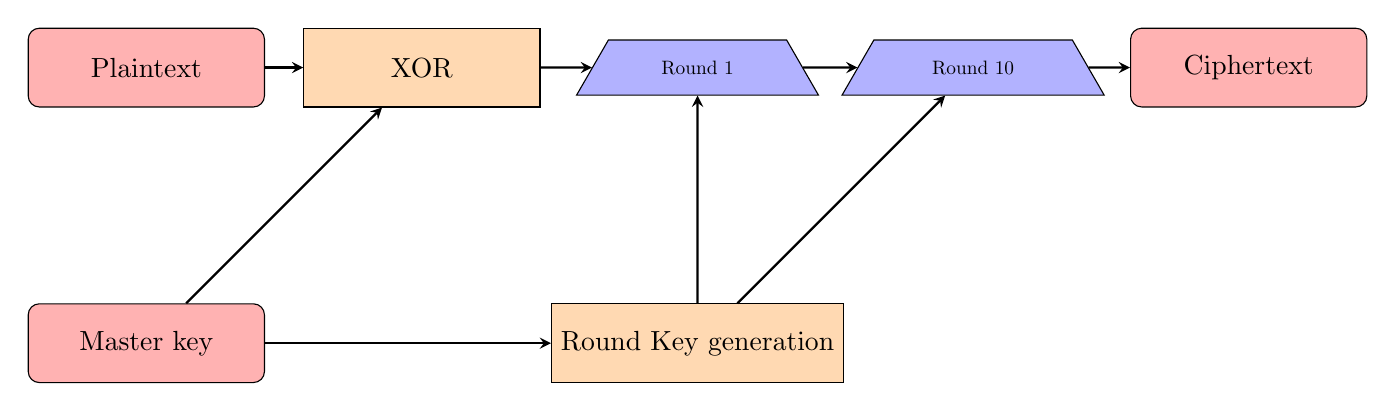
\begin{tikzpicture}[node distance=2cm]
\node (plaintext) [startstop] {Plaintext};
\node (masterkey) [startstop, below of = plaintext, yshift=-1.5cm] {Master key};
\node (XOR) [process, right of = plaintext, xshift=1.5cm] {XOR};
\node (Roundfirst) [io, right of = XOR, xshift=1.5cm, scale=0.7] {Round 1};
\node (Roundlast) [io, right of = Roundfirst, xshift=1.5cm, scale=0.7] {Round 10};
\node (Ciphertext) [startstop, right of = Roundlast, xshift=1.5cm] {Ciphertext};
\node (RoundKey) [process, below of = Roundfirst, yshift=-1.5cm] {Round Key generation};
\draw [arrow] (plaintext) -- (XOR);
\draw [arrow] (XOR) -- (Roundfirst);
\draw [arrow] (Roundfirst) -- (Roundlast);
\draw [arrow] (Roundlast) -- (Ciphertext);
\draw [arrow] (masterkey) -- (RoundKey);
\draw [arrow] (masterkey) -- (XOR);
\draw [arrow] (RoundKey) -- (Roundfirst);
\draw [arrow] (RoundKey) -- (Roundlast);
\end{tikzpicture}
\end{adjustbox}
\end{frame}

\begin{frame}
\frametitle{AES: Rounds}
\begin{adjustbox}{max totalsize={.9\textwidth}{.7\textheight},center}
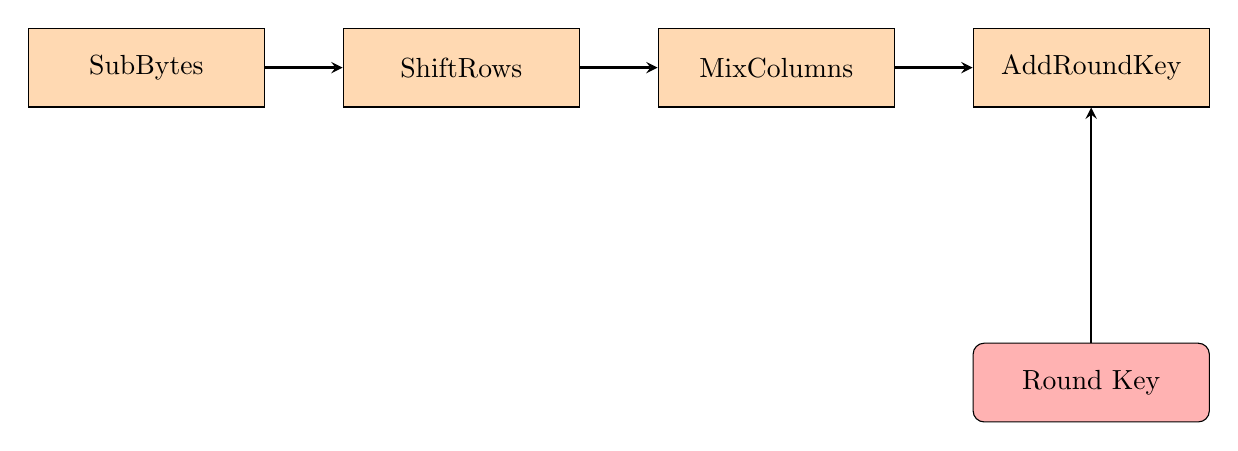
\begin{tikzpicture}[node distance=4cm]
\node (subbytes) [process] {SubBytes};
\node (ShiftRows) [process, right of = subbytes] {ShiftRows};
\node (MixColumns) [process, right of = ShiftRows] {MixColumns};
\node (AddRoundKey) [process, right of = MixColumns] {AddRoundKey};
\node (RoundKey) [startstop, below of = AddRoundKey] {Round Key};
\draw [arrow] (subbytes) -- (ShiftRows);
\draw [arrow] (ShiftRows) -- (MixColumns);
\draw [arrow] (MixColumns) -- (AddRoundKey);
\draw [arrow] (RoundKey) -- (AddRoundKey);
\end{tikzpicture}
\end{adjustbox}
\end{frame}

\begin{frame}
\frametitle{AES: SubBytes}
\begin{center}
\includegraphics<1>[scale=0.45]{SBox.PNG}
\end{center}
\begin{itemize}
\item<2-> Bytewise operation
\item<2-> Sole source of Confusion; the only non-linear operation in AES (affine transformation)
\item<2-> Key-independence is accepted in return for non-linearity; this eliminates one of DES' major weaknesses
\item<2-> Utilization of the multiplicative inverse: if $a \cdot b = 1$ then $b = a^{-1}$
\item<2-> Maximizes non-linearity, but negatively impacts diffusion: $0^{-1} = 0$ and $1^{-1}=1$
\end{itemize}
\end{frame}

\begin{frame}
\frametitle{AES: ShiftRows}

\[ \left( \begin{array}{cccc}
a_{0,0} & a_{0,1} & a_{0,2} & a_{0,3} \\[0pt]
a_{1,0} & a_{1,1} & a_{1,2} & a_{1,3} \\[0pt]
a_{2,0} & a_{2,1} & a_{2,2} & a_{2,3} \\[0pt]
a_{3,0} & a_{3,1} & a_{3,2} & a_{3,3}\end{array} \right)
\xrightarrow{\text{ShiftRows}}
\left( \begin{array}{cccc}
a_{0,0} & a_{0,1} & a_{0,2} & a_{0,3} \\[0pt]
a_{1,1} & a_{1,2} & a_{1,3} & a_{1,0} \\[0pt]
a_{2,2} & a_{2,3} & a_{2,0} & a_{2,1} \\[0pt]
a_{3,3} & a_{3,0} & a_{3,1} & a_{3,2}\end{array} \right)
\]

\pause

\begin{itemize}
\item One of the two primary sources of diffusion
\item One small change to the plaintext should result in a large change to the ciphertext
\item Bytes are placed into the state in column order, but shifted across rows
\end{itemize}
\end{frame}

\begin{frame}
\frametitle{AES: MixColumns}

\[ \left( \begin{array}{cccc}
02 & 03 & 01 & 01 \\
01 & 02 & 03 & 01 \\
01 & 01 & 02 & 03 \\
03 & 01 & 01 & 02\end{array} \right)
\cdot
\left( \begin{array}{c}
a_0 \\
a_1 \\
a_2 \\
a_3\end{array} \right)
=
\left( \begin{array}{c}
s_0 \\
s_1 \\
s_2 \\
s_3\end{array} \right)
\]

\begin{columns}
\begin{column}{0.5\textwidth}
\pause
\begin{center}
$
s_0 = {02}a_0+{03}a_1+{01}a_2+{01}a_3 \\[0pt]
s_1 = {01}a_0+{02}a_1+{03}a_2+{01}a_3 \\[0pt]
s_2 = {01}a_0+{01}a_1+{02}a_2+{03}a_3 \\[0pt]
s_3 = {03}a_0+{01}a_1+{01}a_2+{02}a_3 \\[0pt]
$
\end{center}
\end{column}
\begin{column}{0.5\textwidth}
\begin{itemize}
\pause
\item Each new byte is dependent on an entire column of four old bytes
\item Second source of diffusion
\end{itemize}
\end{column}
\end{columns}
\end{frame}


\begin{frame}
\frametitle{AES: AddRoundKey}
\begin{itemize}
\item Identical to the initialing XOR
\item XORs the round key with the state
\end{itemize}
\begin{center}
\[ 
\left( \begin{array}{cccc}
a_{0,0} & a_{0,1} & a_{0,2} & a_{0,3} \\
a_{1,0} & a_{1,1} & a_{1,2} & a_{1,3} \\
a_{2,0} & a_{2,1} & a_{2,2} & a_{2,3} \\
a_{3,0} & a_{3,1} & a_{3,2} & a_{3,3}\end{array} \right)
\bigoplus
\left( \begin{array}{cccc}
k_{0,0} & k_{0,1} & k_{0,2} & k_{0,3} \\
k_{1,0} & k_{1,1} & k_{1,2} & k_{1,3} \\
k_{2,0} & k_{2,1} & k_{2,2} & k_{2,3} \\
k_{3,0} & k_{3,1} & k_{3,2} & k_{3,3}\end{array} \right)
\]
\end{center}
\end{frame}

\section{A Historical Transition}

\subsection{Conflicts Throughout History}

\begin{frame}
\frametitle{The Crypto War: Past and Present}
\begin{itemize}
\item<2-> WWII: British Special Operations Executive
\item<3-> Value of information: Rising exponentially alongside globalization
\item<4-> Covert operations and proxy wars
\end{itemize}
\begin{columns}
\begin{column}{0.5\textwidth}
\begin{center}
\uncover<5->{
\includegraphics[scale=0.1]{NSA.PNG}}
\end{center}
\end{column}
\begin{column}{0.5\textwidth}
\begin{center}
\uncover<5->{
\includegraphics[scale=0.1]{SVRRF.PNG}}
\end{center}
\end{column}
\end{columns}
\end{frame}

\begin{frame}
\frametitle{Motivator for more Powerful Computing}
\begin{itemize}
\item<2-> Cryptologists vs. Cryptanalysts
\item<3-> Speed and Efficiency: RAM (Rapid Analytic Machines)
\item<4-> Each different problem required a specialized RAM
\item<5-> Alan Turing's Thesis: Build a computer not restricted to one specific problem
\item<6-> Colossus: The world's first programmable computer
\end{itemize}
\begin{center}
\uncover<6->{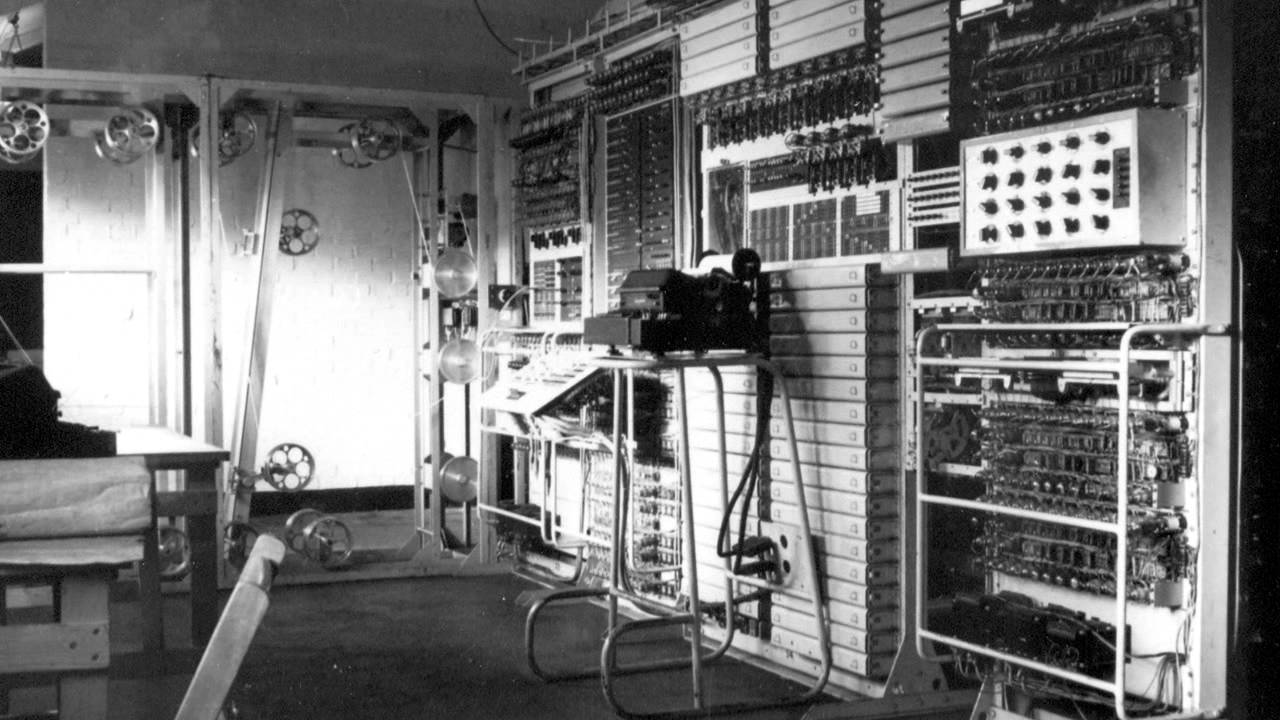
\includegraphics[scale=0.15]{colossus.jpg}}
\end{center}
\end{frame}

\begin{frame}
\frametitle{Today's Issues}

\begin{columns}
\begin{column}{0.5\textwidth}
\begin{itemize}
\item<1-> Mode of operation: ECB
\item<3-> Goal for security purposes: Pseudo-random result
\item<4-> Other modes of operation: CBC (Cipher Block Chaining)
\item<4-> A variety of systems are necessary; key exchange
\end{itemize}
\end{column}
\begin{column}{0.5\textwidth}
\includegraphics<1>[scale=0.7]{tux.jpg}
\includegraphics<2>[scale=0.7]{tux_ecb.jpg}
\includegraphics<3->[scale=0.7]{tux_secure.jpg}
\end{column}
\end{columns}
\end{frame}

\begin{frame}
\begin{center}
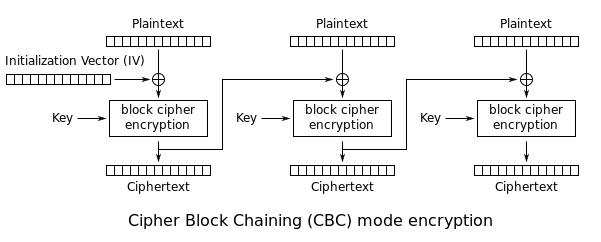
\includegraphics[scale=0.5]{CBC.PNG}
\end{center}
\end{frame}

\subsection{Cryptography in Our Society}

\begin{frame}
\frametitle{New Possibilities and new Risks}
\begin{columns}
\begin{column}{0.5\textwidth}
\begin{itemize}
\item<2-> Technology and social media are becoming ever more linked with our daily lives
\item<3-> Multiple protocols and algorithms are integral to the security of your data
\item<3-> Insecure or compromised data can be easily accessed
\end{itemize}
\end{column}
\begin{column}{0.5\textwidth}
\uncover<2->{
\includegraphics[scale=0.1]{SocialMedia.PNG}} \break
\uncover<3->{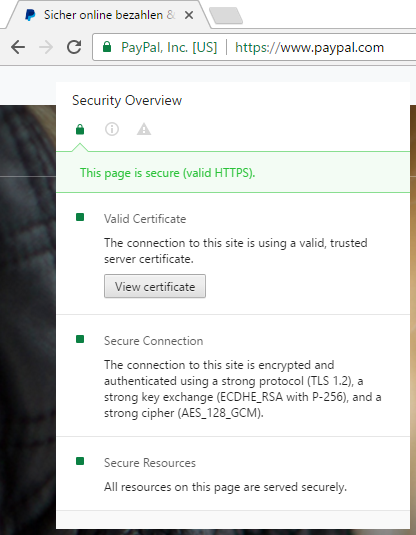
\includegraphics[scale=0.3]{https.PNG}}
\end{column}
\end{columns}
\end{frame}

\begin{frame}
\frametitle{Mass surveillance}
\begin{columns}
\begin{column}{0.5\textwidth}
\begin{center}
\includegraphics<2->[scale=0.1]{snowden.jpg}
\end{center}
\end{column}
\begin{column}{0.5\textwidth}
\begin{center}
\includegraphics<2->[scale=0.2]{BoundlessInformant.PNG}
\end{center}
\end{column}
\end{columns}
\begin{itemize}
\item<3-> 3 billion data elements were collected over 30 days in the US alone
\item<3-> Data collection took place worldwide, including phone call metadata
\item<3-> Data collection and storage is still active
\end{itemize}
\end{frame}

\begin{frame}
\frametitle{Privacy: An Outdated Concept?}
\begin{center}

\includegraphics[scale=0.3]{termsandconditions.png}
\end{center}
\begin{itemize}
\item<2-> Historically academic subject
\item<2-> Thrust into the public eye through recent revelations
\item<2-> Highly relevant to the daily lives of regular people for the first time
\end{itemize}
\end{frame}

\section{Questions}

\begin{frame}
\frametitle{Questions}
\begin{center}
\Huge{?}
\end{center}
\end{frame}

 

\end{document}